\documentclass[twocolumn]{article}

% -----------------------------------------------------------------------------------

% choose options for [] as required from the list % in the
% Reference Guide
\usepackage[a4paper, left=1cm, right=1cm, top=1in, bottom=1in]{geometry}

\usepackage{mathptmx}       % selects Times Roman as basic font
\usepackage{helvet}         % selects Helvetica as sans-serif font
\usepackage{courier}        % selects Courier as typewriter font
\usepackage{type1cm}        % activate if the above 3 fonts are
                            % not available on your system
%
\usepackage{makeidx}         % allows index generation
\usepackage{graphicx}        % standard LaTeX graphics tool
                             % when including figure files
\usepackage{multicol}        % used for the two-column index
\usepackage{seqsplit}
\graphicspath{{Figure/}}

% -----------------------------------------------------------------------------------
\usepackage{amsmath}
\usepackage{amsfonts}        % for sets like \mathbb{N}, \mathbb{Z}, etc.
\usepackage{amssymb}         % for symbols like \therefore, \because, etc.
\usepackage{amsthm}          % for theorems, definitions, etc.
\usepackage{mathtools}       % for \coloneqq, \eqqcolon, etc.

\usepackage{bm}              % for bold symbols
\usepackage{caption}         % for controlling figure/table captions
\usepackage{float}           % to improve figure positioning

\usepackage{microtype}
\usepackage[none]{hyphenat} % Prevents hyphenation
\sloppy % Allows LaTeX to be less strict about line breaking


\usepackage{hyperref}
% \usepackage{apacite}
\usepackage[style=numeric, backend=biber]{biblatex}
\addbibresource{references.bib}


\usepackage{enumitem} 
\usepackage[small,compact]{titlesec} 
\titlespacing{\section}{0pt}{*4}{*1.5}

\usepackage{setspace}
\edef\restoreparindent{\parindent=\the\parindent\relax}
\usepackage{parskip}
\restoreparindent

\usepackage{titlesec}
\titlespacing*{\section}{0pt}{20pt}{5pt} % No space above or below \section

\usepackage[skip=0pt]{caption} % Remove space around captions

% % Adjust global float spacing
% \setlength{\textfloatsep}{0pt}
% \setlength{\abovecaptionskip}{0pt}
% \setlength{\belowcaptionskip}{0pt}
% -----------------------------------------------------------------------------------

% \DefineBibliographyStrings{english}{
%   andothers = {et al} % Removes the period after "et al"
% }

%%%%%%%%%%%%%%%%%%%%%%%%%%%%%%%%%%%%%%%%%%%%%%%%%%%%%%%%%%%%%%%%%%%%%%%%%%%%%%%%%%%%%%%%%


\setlength{\columnsep}{1cm} % Adjust column separation
\title{STUDY ON WARNING OF QUEENLESS \break BEE HIVE BASED ON SOUND CLASSIFICATION}
\author{\normalsize Khoi Nguyen Dao, Hoang Le Nguyen, Anh Tuan Hoang Nguyen, Son Trung Nguyen}
\date{\normalsize Hanoi University of Science and Technology, Vietnam}

\begin{document}
\maketitle

% Abstract
\input{Sections/abstract.tex}

% Introduction
\section{Introduction}
In beekeeping, the queen bee plays a vital role in maintaining the stability and development
of the bee colony. The queen is the reproductive center of the colony, and she also regulates
the activities and social structure within the hive \cite{anton2022introduction}. The loss of the queen bee
often leads to serious consequences such as reduced reproductive capacity, an imbalance in
colony activities, and can even lead to the complete collapse of the bee colony. Therefore,
early detection and warning of abnormal queen bee loss in beehives is crucial to ensure
production efficiency and maintain the health of the bee colony.

If the loss of the queen bee in the colony is not detected promptly, it can cause serious
problems such as an imbalance in the activities of the hive, leading to disorientation and
chaos, resulting in a decline in the bee population, leading to the weakening and eventual
death of the entire bee colony \cite{honey_bee_colony_2021}. Therefore, the need for a device to provide early
warning of queen loss is very important to help beekeepers intervene promptly. A warning
system can quickly detect the loss of the queen, allowing beekeepers to intervene by
replacing the queen with a new one or stimulating the colony to create a new queen before
the colony weakens, thus reducing the damage caused by the loss of the queen.


% Related Work
\section{Related Work}
The development of Artificial Intelligence (AI) is opening up new opportunities for the
beekeeping industry. AI technology allows for efficient remote monitoring, collecting
continuous data on various aspects of bee colony life. AI algorithms are applied to analyze
and process data, providing accurate information about the health and activity of bee
colonies. This enables beekeepers to monitor their colonies 24/7 without direct
intervention, detecting and addressing problems such as diseases or other harmful
factors in a timely manner. Consequently, they can optimize beekeeping, improve product
yield and quality, and save time and costs in colony management. Although this technology
has been widely researched and applied in many countries worldwide, the application of AI
in beekeeping in Vietnam is still limited. Research related to the detection of anomalies
in beekeeping can be mentioned as follows:

Several systems introduced by
\citeauthor{schurischuster2016sensor} (\citeyear{schurischuster2016sensor}) \cite{schurischuster2016sensor},
\citeauthor{zacepins2016remote} (\citeyear{zacepins2016remote}) \cite{zacepins2016remote},
\citeauthor{antonio2017frequency} (\citeyear{antonio2017frequency}) \cite{antonio2017frequency},
\citeauthor{crawford2017automated} (\citeyear{crawford2017automated}) \cite{crawford2017automated}
have used a multi-sensor beehive monitoring system
called BeePi, including a Raspberry Pi computer, a miniature camera, 4 microphones connected
to a splitter, a solar panel, a temperature sensor, a battery, and a clock. In the research
of \citeauthor{kulyukin2018toward} \cite{kulyukin2018toward}, microphones were placed to collect sound samples of bees,
crickets, and ambient noise. The authors then used machine learning models on bee sound
datasets collected from different locations to train and classify the collected sounds.
The experimental results achieved high accuracy, so it is entirely possible to use sound
to monitor the hive status.

Besides the above research on bee monitoring, in 2019, research by Ruvinga and colleagues
used the MFCC feature extraction method along with a CNN network to predict queen bee loss
sounds with an accuracy rate of up to 99\% on the Arnia Ltd. dataset
(\citeurl{ruvinga2023identifying}) \cite{ruvinga2023identifying},
which shows that beehive sound analysis technology has been used as an effective tool for
early detection of problems related to the queen bee, especially the loss of the queen. One
of the reasons why sound analysis is an effective tool for early detection of problems
related to the queen bee is that the transformation and change of sound are obvious when
the queen bee of the bee colony has a problem, for example: When the queen bee dies or
leaves, the hive sound can change from a quiet and rhythmic state to abnormal sounds such
as long and repetitive buzzing of worker bees. This characteristic sound is a clear sign of
instability in the hive. Compared to other inspection methods such as temperature or
humidity sensors, although temperature or humidity sensors can detect changes in the bee
colony environment, they cannot provide specific information about the status of the queen
bee or the bee colony. Sound analysis will have clearer data on queen loss based on the
activity and behavior of worker bees.

Based on the analysis of research on detection monitoring in the beekeeping process,
and then providing analysis to warn of queen loss, the research team chooses to
analyze the sound collected from the beehive to issue an early warning of queen loss for
deployment. This method provides high accuracy and is easy to automate, helping beekeepers
monitor their bee colonies continuously and reduce risks. Compared to other monitoring
methods, sound analysis not only detects early queen loss but also helps protect the health
of the bee colony without direct intervention in the hive.

In essence, this text discusses the application of AI, particularly sound analysis, in
beekeeping to detect problems like queen bee loss. It highlights the advantages of using
AI, such as remote monitoring, early detection, and improved efficiency. The text also
provides examples of existing research and the benefits of using sound analysis over other
methods.


% Theoretical Foundation for Anomaly Detection in Sound Classification
\section{Theoretical Foundation for Anomaly Detection in Sound Classification}
According to the chosen problem-solving approach, our research team will extract sound
features and make predictions following the process shown in the image:

\vspace{-1em}
\begin{figure}[H]
  \centering
  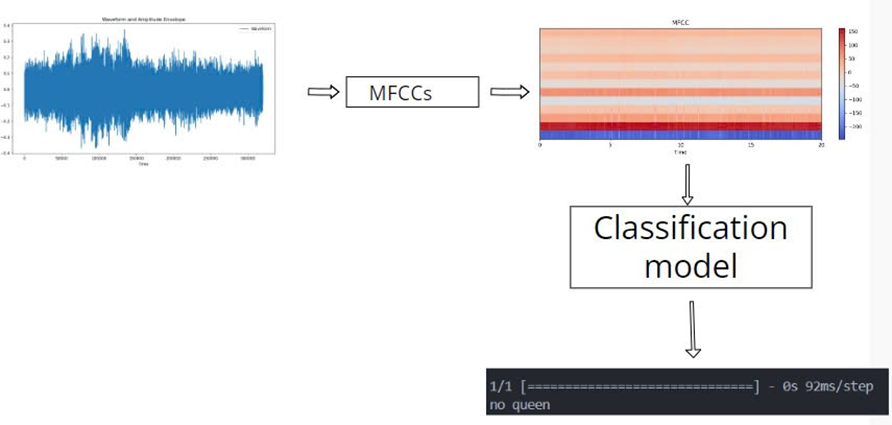
\includegraphics[width=0.47\textwidth]{Audio-Classification-Process.png}
  \caption{Audio Classification Process}
  \label{fig:audio-classification-process}
\end{figure}
\vspace{-1em}

In this process, the audio file will go through the MFCC feature extraction step to
transform from the time domain to the frequency domain. Afterward, the classification
model will output the result indicating whether the audio file contains a queen bee or not.
The two classification models we used are the Convolutional Neural Network (CNN) and the
Long Short-Term Memory (LSTM) combined with CNN (LSTM+CNN).


% Feature Extraction in Audio
\section{Feature Extraction in Audio}

To extract features from audio, we use the MFCC
(Mel-Frequency Cepstral Coefficients) technique and
spectrograms to visualize the audio. The audio feature
extraction process will include steps such as Pre-emphasis,
Windowing, DFT (Discrete Fourier Transform), etc.\cite{hossan2011novel}, as follows:

\vspace{-1em}
\begin{figure}[H]
    \centering
    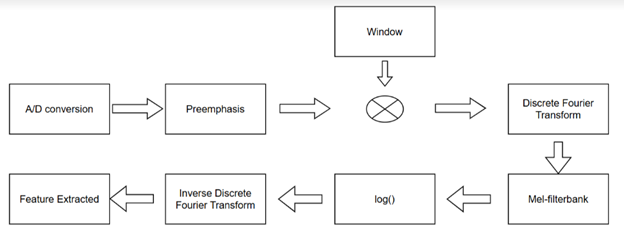
\includegraphics[width=0.47\textwidth]{Audio-Feature-Extraction-Steps.png}
    \caption{Audio Feature Extraction Steps}
    \label{fig:audio-feature-extraction-steps}
\end{figure}
\vspace{-1em}

\subsection{Pre-emphasis}

Pre-emphasis is a signal processing technique commonly used
in the context of audio and speech processing. It is applied
to the input audio signal before proceeding with subsequent
processing steps, such as calculations in MFCC. The purpose of
pre-emphasis is to emphasize higher frequencies in the audio
signal, which often have lower energy compared to lower
frequencies. This helps improve the Signal-to-Noise Ratio
(SNR) and enhance the clarity of speech or other audio
signals, especially in subsequent processing steps.

Mathematically, pre-emphasis is performed as a high-pass
filter between high frequencies compared to lower frequencies.
Typically, it is performed using a first-order FIR
(Finite Impulse Response) filter with a simple equation:

\vspace{-1em}
\begin{equation}
    y[n] = x[n] - \alpha \cdot x[n-1]
\end{equation}
\vspace{-1em}

Where:
\begin{itemize}
    \item $y(n)$: Output signal after pre-emphasis.
    \item $x(n)$: Input audio signal.
    \item $\alpha$: Pre-emphasis coefficient in the range from 0.9 to 0.97.
\end{itemize}

This filter operates by subtracting a scaled version of the
previous sample from the current sample, effectively
amplifying high-frequency components and attenuating
low-frequency components. This compensates for the spectral
tilt typically observed in speech and other audio signals,
resulting in a flatter frequency response and improved
intelligibility.

\subsection{Windows}

Instead of performing a Fourier transform on the entire long
audio segment, we slide a window along the signal to extract
smaller audio segments and then apply the DFT to each of these
segments. However, each window should be divided into three
parts: pre-emphasis, the current segment, and post-emphasis.
This helps avoid losing information from each extracted audio
segment. Each window also needs to overlap to better preserve
information; typically, windows overlap by about $10ms$.

\vspace{-1em}
\begin{figure}[H]
    \centering
    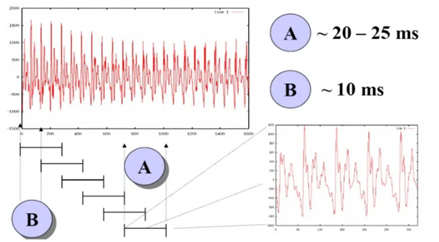
\includegraphics[width=0.47\textwidth]{Windowing-Technique-for-Audio-Signals.png}
    \caption{Windowing Technique for Audio Signals}
    \label{fig:windowing-technique-for-audio-signals}
\end{figure}
\vspace{-1em}

\subsection{Discrete Fourier Transform and Spectrograms:}

Using the Fourier transform, a time-domain signal can be
transformed into its frequency-domain representation. This
transformation provides information about the frequency
content of the signal, including both the frequencies present
and their corresponding magnitudes.

\vspace{-1em}
\begin{figure}[H]
    \centering
    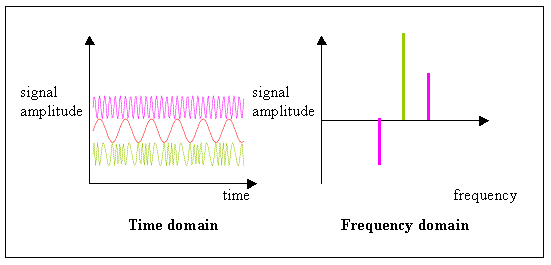
\includegraphics[width=0.47\textwidth]{Fourier-Transform-of-a-Sound-Signal.png}
    \caption{Fourier Transform of a Sound Signal \cite{technical_editor_2017}.}
    \label{fig:fourier-transform-of-a-sound-signal}
\end{figure}
\vspace{-1em}

The Fourier transform provides a frequency-domain
representation of the signal, resulting in a magnitude
spectrum. However, this transformation inherently loses time
localization information, making it impossible to determine
the temporal occurrence of specific frequency components. To
overcome this limitation, a time-frequency representation is
required, which is provided by the spectrogram. In a
spectrogram, the abscissa represents time, the ordinate
represents frequency, and the color intensity represents the
magnitude of the spectral components. Higher color intensity
corresponds to higher magnitudes (stronger frequency components).

\vspace{-1em}
\begin{figure}[H]
    \centering
    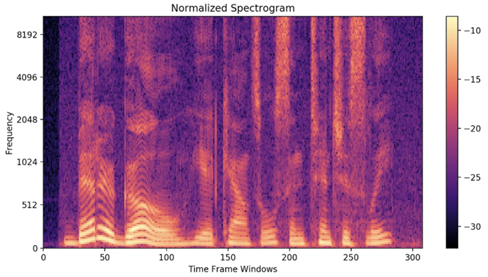
\includegraphics[width=0.47\textwidth]{Spectrogram-after-applying-Fourier-transform.png}
    \caption{Frequency Spectrum after Fourier Transform}
    \label{fig:spectrogram-after-applying-fourier-transform}
\end{figure}
\vspace{-1em}

The Discrete Fourier Transform (DFT) is mathematically defined
as:

\begin{equation}
    X[k] = \sum_{n=0}^{N-1} x[n] \cdot e^{-i \frac{2\pi}{N}kn}
\end{equation}

Where:
\begin{itemize}
    \item $X[k]$: Represents the complex-valued amplitude of the
          $k^{th}$ frequency component in the frequency domain. It's
          often referred to as the $k^{th}$ "frequency bin" or "spectral
          component".

    \item $x[n]$: Denotes the $n^{th}$ sample of the input signal
          in the time domain.

    \item $N$: Is the total number of samples in the input
          signal being analyzed.

    \item $k$: Is the frequency index, taking integer values
          from $0$ to $N-1$. These values correspond to discrete
          frequencies ranging from $0$ Hz to $\frac{(N-1)}{N}$ times the
          sampling frequency. The maximum frequency (when $k = \frac{N}{2}$
          for even $N$) is known as the Nyquist frequency.

    \item $j$: Represents the imaginary unit, defined as $\sqrt{-1}$.
          This indicates that $X[k]$ is a complex number with both
          real and imaginary parts (or magnitude and phase).

    \item $n$: Is the sample index in the time domain,
          iterating from $0$ to $N-1$ within the summation.

    \item $k$: Is the frequency index, indicating which
          frequency component is being computed.

\end{itemize}

In essence, the DFT is a crucial step in MFCC extraction,
transforming the time-domain input signal into its frequency-
domain representation. This decomposition into individual
frequency components facilitates the creation of a spectrogram,
a visual representation of the signal's frequency content over
time. This representation simplifies subsequent machine
learning tasks by providing relevant features in a more
manageable and informative form.

\subsection{Mel-filterbank}
The human auditory system exhibits a non-linear frequency
response, demonstrating greater sensitivity to changes in
lower frequencies and reduced sensitivity to changes in higher
frequencies. The Mel filterbank is designed to model this
perceptual non-linearity, providing a perceptually relevant
representation of the audio signal.

The Mel scale is a psychoacoustic scale of perceived pitch
based on human auditory perception. It is characterized by a
non-linear relationship with linear frequency (Hz), with a
greater emphasis on the lower frequency region.

The conversion from linear frequency (Hertz) to Mel frequency
is often done using a formula like this:

\begin{equation}
    f_{mel} = 2595 \cdot \log\left(1 + \frac{f}{500}\right)
\end{equation}

The Mel filterbank operates on the power spectrum of an audio
signal. The power spectrum provides a representation of the
signal's energy distribution across discrete frequency bins.
Each triangular filter of the Mel filterbank is convolved with
the power spectrum, yielding a series of filter bank outputs.

\vspace{-1em}
\begin{figure}[H]
    \centering
    \includegraphics[width=0.47\textwidth]{Mel-Filterbank.png}
    \caption{Mel-filterbank}
    \label{fig:mel-filterbank}
\end{figure}
\vspace{-1em}

The filter bank outputs represent an approximation of the
signal's energy distribution across various frequency bins,
with higher output magnitudes signifying greater energy
concentration within the corresponding frequency bins. These
outputs capture the signal's energy distribution across
different frequency bands in a perceptually significant
manner.

Squaring the magnitude spectrum obtained from the DFT,
followed by the application of a Mel-scale filterbank across
the frequency axis, results in each filter output representing
the integrated energy within its corresponding Mel-scaled
frequency band. The resulting representation is referred to as
the Mel-scale spectrum.

\vspace{-1em}
\begin{figure}[H]
    \centering
    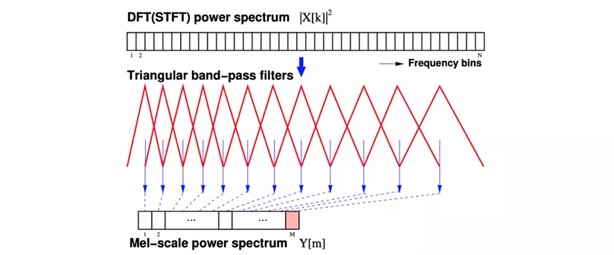
\includegraphics[width=0.47\textwidth]{Mel-Scale-Conversion-of-the-DFT-Spectrum.png}
    \caption{Mel-Scale Conversion of the DFT Spectrum \cite{nacem2020subspace}}
    \label{fig:mel-scale-conversion-of-the-dft-spectrum}
\end{figure}
\vspace{-1em}

\subsection{log()}

The role of the logarithm function in calculating
Mel-Frequency Cepstral Coefficients (MFCCs) is to compress
the dynamic range of the filter output values. Logarithmic
compression helps make the MFCC representation more robust to
variations in signal intensity and enhances its discriminative
ability.

Assuming an input signal $x$ with impulse response $h$, the
resulting audio spectrum in terms of sound intensity is:

\begin{equation}
    |Y(w)| = |X(w)| \cdot |H(w)|
\end{equation}

After applying the logarithm, we obtain:

\begin{equation}
    \log|Y(w)| = \log|X(w)| + \log|H(w)|
\end{equation}

\subsection{Discrete Cosine Transform (DCT)}

The Discrete Cosine Transform (DCT) constitutes the final
stage of MFCC feature extraction. The fundamental concept
behind the DCT is analogous to that of the Inverse Discrete
Fourier Transform (IDFT). Following MFCC feature extraction,
a transformation from the frequency domain to the time domain
is conducted. The MFCC representation typically utilizes the
first $12$ coefficients obtained from the IDFT, augmented with
the energy term, as its characteristic features.

\vspace{-1em}
\begin{figure}[H]
    \centering
    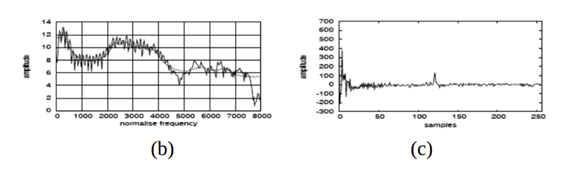
\includegraphics[width=0.47\textwidth]{Time-Domain-Signal-Reconstructed-from-IDFT.png}
    \caption{Time-Domain Signal Reconstructed from IDFT}
    \label{fig:time-domain-signal-reconstructed-from-idft}
\end{figure}
\vspace{-1em}

The dominant frequency observed at the center of
\autoref{fig:time-domain-signal-reconstructed-from-idft}c
corresponds to $F_0$, the fundamental frequency of the acoustic 
signal. $F_0$ serves as a distinguishing characteristic of an 
individual's voice pitch. The leftmost region of the figure 
represents phonetic information associated with the formants 
$F_1$, $F_2$, etc. Within the context of sound classification, the 
fundamental frequency $F_0$ and the formant frequencies $F_1$, $F_2$, $F3$, 
and so forth, constitute important features for speaker 
characterization.

\subsection{Dynamic features}

The MFCC process results in $39$ features, of which the first $12$ 
are obtained by applying the DCT (Discrete Cosine Transform) 
to the $\log$ Mel spectrum. The $13^{th}$ feature is the energy of 
each time frame. The remaining $26$ features are divided into 
two sets of $13$ features each. The first set of $13$ features is 
used to calculate the first-order derivatives (delta 
coefficients), and the last $13$ features are used to calculate 
the second-order derivatives (delta-delta coefficients) at 
time $x$:

\begin{equation}
    f'(x) = \frac{f(x + \Delta t) - f(x - \Delta t)}{2\Delta t}
\end{equation}

\begin{equation}
    f''(x) = \frac{f'(x + \Delta t) - f'(x - \Delta t)}{2\Delta t}
\end{equation}

By calculating the first-order and second-order derivatives 
of MFCCs or other feature vectors, the temporal dynamics and 
variations within the signal can be captured, providing 
additional information that can be useful for tasks such as 
speech recognition, speaker recognition, and emotion 
recognition. These derivatives can be concatenated with the 
original feature vectors to create extended feature 
representations to improve performance in such tasks.


% Proposed Machine Learning Models
\section{Proposed Machine Learning Models}
Our research team proposes using two popular architectures:
Convolutional Neural Networks (CNNs) and a combination of
Long Short-Term Memory networks with CNNs. Each model has its own
advantages and disadvantages that need to be considered.

\vspace{1em}
\begin{figure}[H]
    \centering
    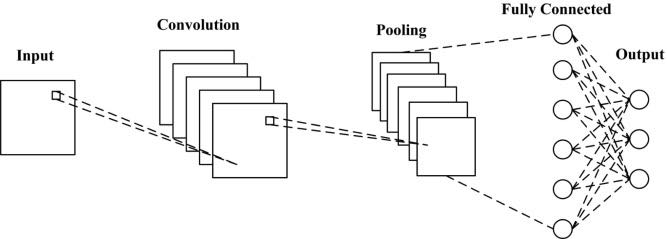
\includegraphics[width=0.47\textwidth]{CNN-model.jpg}
    \caption{CNN Model}
    \label{fig:cnn-model}
\end{figure}
\vspace{1em}

Convolutional Neural Networks (CNNs) (\autoref{fig:cnn-model}) are a powerful tool for extracting spatial
features from audio data. When audio is converted into spectrograms, which visually
represent sound, CNNs can identify local patterns like edges and textures in the data \cite{oshea2015introduction}.
One of the biggest advantages of CNNs is their translational invariance, which makes the
model resistant to shifts and distortions in the input data. Moreover, CNNs significantly
reduce the number of parameters by sharing weights, making the training process more
efficient. This model is also easily scalable by adding more layers and filters, allowing
for the extraction of increasingly complex features.

Research group proposed a CNN model begins with an input layer
designed to accept an input image. It first applies a 2D
convolutional layer with 32 filters, a 3x3 kernel size, and ReLU
activation, followed by a max pooling layer with a 2x2 pool size and
strides of 2x2 to downsample the feature maps. The process is repeated
with a second convolutional layer, this time with 64 filters and the
same kernel size and activation, followed by another max pooling layer
with identical parameters. The feature maps are then flattened into a
1D vector, which is passed through a series of fully connected (dense)
layers. The first dense layer has 64 units with ReLU activation,
followed by a second dense layer with 250 units and ReLU activation,
and a third dense layer with 100 units and ReLU activation. This model
concludes with an output dense layer containing a single unit with a
sigmoid activation function for binary classification tasks.

However, CNNs have some limitations. The model primarily captures spatial features and may
not be effective in capturing the temporal dependencies inherent in sequential
audio data \cite{lim2020time}. CNNs also require a fixed input size, which can be a limitation when
processing audio segments of varying lengths. Additionally, audio data needs to be
converted into spectrograms or other image-like representations before being fed into a CNN,
requiring an additional preprocessing step.

\vspace{-1em}
\begin{figure}[H]
    \centering
    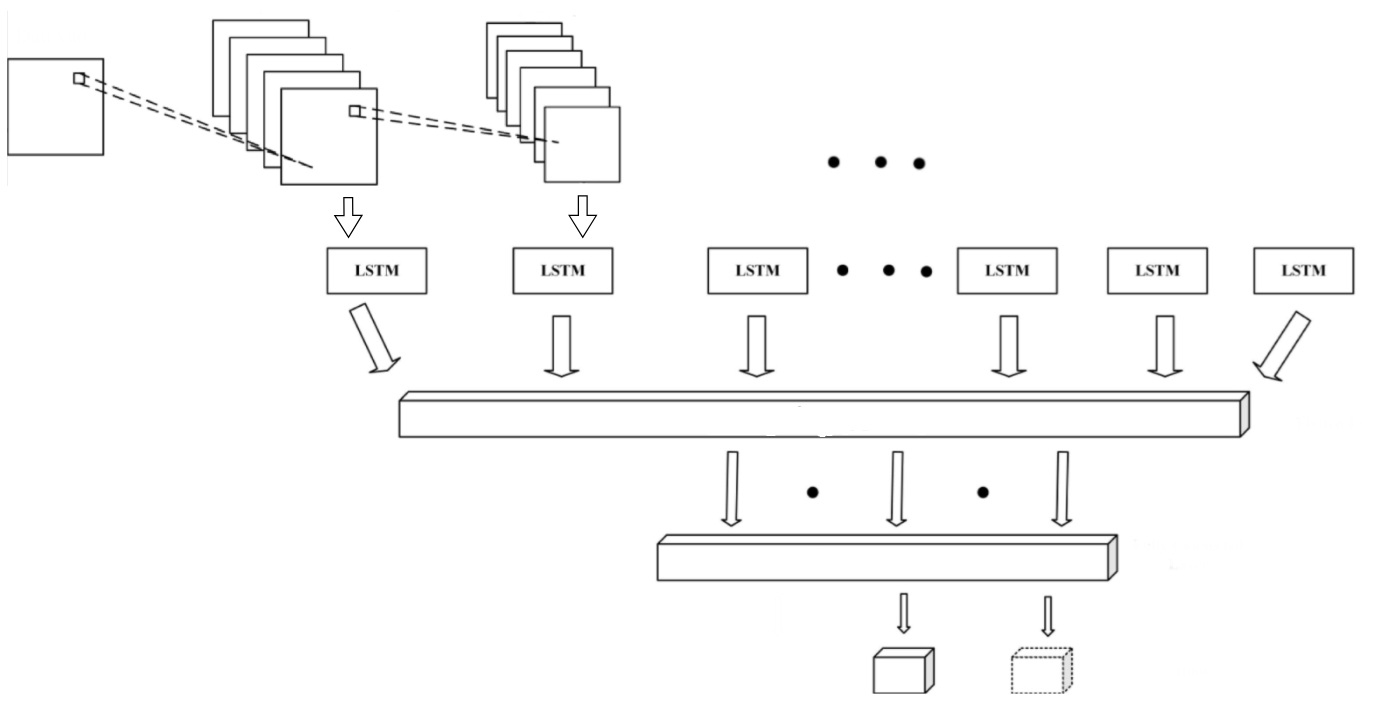
\includegraphics[width=0.47\textwidth]{LSTM-CNN-model.png}
    \caption{LSTM+CNN Model}
    \label{fig:lstm-cnn-model}
\end{figure}
\vspace{-1em}

In this study, we utilize a hybrid LSTM+CNN (\autoref{fig:lstm-cnn-model}) 
model to leverage the strengths of both architectures: the Convolutional Neural Network (CNN) 
for automatic feature extraction from spatial data and the Long Short-Term Memory (LSTM) 
network for capturing temporal dependencies in sequential data. This combined approach is 
designed to enhance model performance on tasks involving both spatial and temporal patterns. 
For a detailed explanation of the LSTM+CNN architecture and its implementation, please refer 
to the Appendix section.

In summary, we have outlined the advantages and disadvantages of our
models, CNN and LSTM+CNN, based on the theoretical foundation. The
evaluation of the performance of the two models, based on accuracy and
computational speed, will be conducted through practical experiments
on the bee audio dataset collected through IoT devices installed by
the group at the bee farm.


% Dataset
\section{Dataset}
Dataset in this research is collected at Vietnam National University of
Agriculture, to record queenless sound we created a queen-absent
situation in the hive: using a number of sample bee boxes, installing
data collection devices (IoT kits), we suddenly removed the queen for a
certain period of time, and then reintroduced the queen into the bee
box. This process was repeated several times, at different weather
conditions. All of this dataset is made by Hoang Le Nguyen and Hieu
Duy Tran from CDiT (https://cdit.ptit.edu.vn/) and it is the result of
"Research and apply technology from Industry 4.0 into production
management of honey for domestic consumption and exportation",
research code: "KC-4.0-20/19-25". \cite{pham2020industry4}

% Experimental Results
\section{Experimental Results}
In this experiment, we conducted tests using the MFCC (Mel-frequency cepstral coefficients)
feature extraction method combined with two neural network models: CNN (Convolutional Neural
Network) and LSTM+CNN (Long Short-Term Memory + Convolutional Neural Network) to identify
bee sounds. The test dataset consisted of 500 untrained audio files collected using IoT
devices installed on Apis mellifera beehives at the Bee Center of the Vietnam National University of Agriculture,
including 405 audio files of bee colonies with queens and 110 files without
queen bees. The experimental results showed that the CNN model achieved an accuracy of
96.29\% (390/405) with a prediction time of 50.97 seconds, while the LSTM+CNN model only
achieved 80.24\% (325/405) accuracy and took 123.78 seconds to process.
The accuracy and processing time measurement in this research is
calculated base on this formular:

\vspace{-1em}
\begin{equation}
  \footnotesize \text{Accuracy}
  = \frac{\footnotesize \text{Number of predicted right} + \text{\footnotesize Number of silent file predicted}}{\small \text{Total number of file}}
\end{equation}
\vspace{-1em}

\vspace{-1em}
\begin{equation}
  \text{Processing time} = \text{\small End process time} - \text{\small Start processing time}
\end{equation}
\vspace{-1em}

The results of the two models are presented in detail in \autoref{tab:model_comparison}:

\vspace{-1em}
\begin{table}[H]
  \centering
  \resizebox{0.47\textwidth}{!}{%
    \begin{tabular}{|c|c|c|}
      \hline
      \textbf{Model} & \textbf{Accuracy} & \textbf{Processing time} \\ \hline
      CNN            & 96.29\%           & 50.97 seconds            \\ \hline
      LSTM+CNN       & 80.24\%           & 123.78 seconds           \\ \hline
    \end{tabular}%
  }
  \caption{Comparison of accuracy and processing time between models}
  \label{tab:model_comparison}
\end{table}
\vspace{-1em}

Analysis of the results shows that the CNN model not only outperforms in terms of accuracy
but also in processing speed, which is nearly 2.5 times faster than LSTM+CNN. The research
results also confirm the effectiveness of combining the MFCC feature extraction method with
the CNN model in the problem of anomaly detection through bee sound classification.
Although the LSTM+CNN model has a more complex structure, in this particular case, the
model does not yield higher performance compared to CNN.

From the experimental results, we can conclude that the combination of the MFCC feature
extraction method and the CNN network is an effective method for identifying bee sounds,
ensuring not only high accuracy but also fast processing speed, making it a good choice
for practical applications in this field.


% Conclusion and Recommendations
\section{Conclusion and Recommendations}
In this paper, we concluded that the AI sound classification system to support early
warning of queen loss will achieve an accuracy of more than 16\% higher and a speed
2.5 times faster when using the MFCC feature extraction technique with the CNN machine
learning model compared to LSTM+CNN. The system uses  sound from beehives, trainning AI
to predict anomalies with MFCCs (to represent sound as images) and CNN
(to extract important features from MFCCs), thereby optimizing bee care, improving
productivity and product quality, and saving time and costs in bee management. The
research group aims to continue researching, designing devices and developing equipment
to analyze and evaluate more abnormal cases in beehives to warn beekeepers such as:
warning of swarm division, insect attacks, diseases, etc.


% Appendix
\section{Appendix}
Combining CNNs and LSTMs (\autoref{fig:lstm-cnn-model}) offers several benefits. The LSTM+CNN model leverages
the strengths of both models, capturing both spatial features (through CNN) and
temporal dependencies (through LSTM) \cite{sainath2015convolutional}.
This makes them suitable for audio classification where temporal patterns are crucial.
This combination often leads to better performance in tasks that require understanding both
local features and global sequence patterns, such as speech recognition and music genre
classification. Moreover, LSTMs can handle variable-length sequences \cite{lim2020time},
making the combined model more flexible in processing audio segments of different lengths.

However, combining CNNs and LSTMs results in more complex models with more parameters,
requiring more computational resources, and training LSTM+CNN models takes longer than
training a standalone CNN.


\printbibliography
\end{document}